\chapter{Mobile robots}
\vspace{-1cm}
\begin{figure}[h]
    \centering
    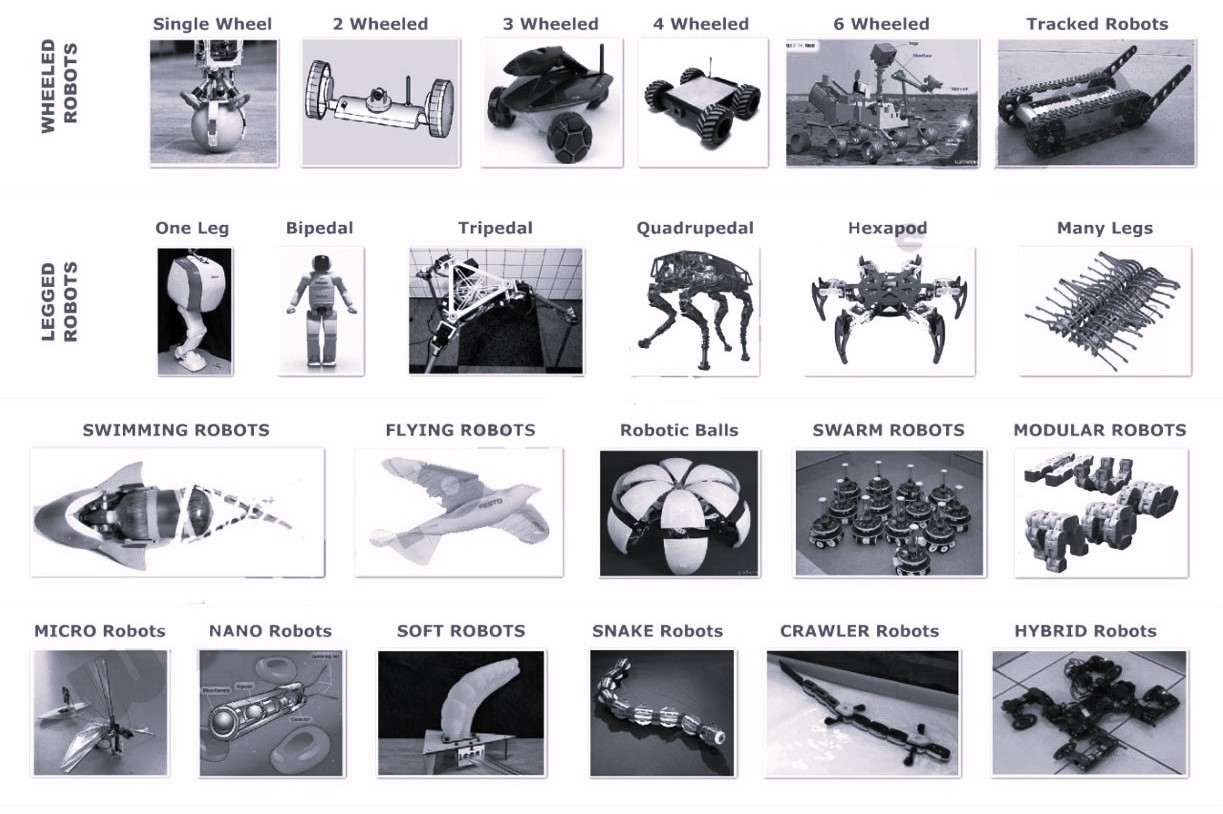
\includegraphics[scale=0.5]{img/classification.jpg}
\end{figure}
\vspace{-0.5cm}
\section{Introduction}
\begin{definition}[\textbf{Mobile robot}]
A \textbf{mobile robot} is a structure capable of moving and act in \textit{terrestrial}, \textit{underwater} or \textit{aerial} environments.    
\end{definition}
\noindent
The characteristics of the environment are fundamental since planning and control are affected by it. Namely the environment can be \underline{totally structured}, \underline{unstructured} or \underline{partially structured}. We refer the \textbf{structuredness} of the environment as the knowledge on geometric characteristics.
\subsection{Autonomy}
A mobile robot is equipped with a certain level of \textbf{autonomy} which makes the structure capable of moving independentlyh from a human supervisor. For achieving it, it is required a computational part (CPU, Intelligence of the robot), some sensors and actuators and an energy source, which can be either generated on-board or provided by mean of an external source.
\subsection{Locomotion}
Another fundamental aspect is that, differently from manipulators, a mobile robot is equipped with a \textbf{locomotion apparatus} which drastically changes according to the environment they are acting in. A \textbf{terrestrial robot} can have wheels, legs or a biomimetic locomotion system; a \textbf{underwater robot} can provided with propellers or water jets; finally, an \textbf{aerial robots} can have rotating, fixed or flapping wings.

\section{Types of wheels}
In the following we are focusing our attention on the wheeled robots, as they represent the great majority of mobile robots used in applications. The basic mechanical structure of this robot is indeed the wheel. The table \Cref{tab:wheels} shows a summary of the fundamental information about the most popular types of wheels.

\begin{table}
    \centering
    \begin{tabular}{m{5cm} m{9cm} m{2cm} }
        \textbf{WHEEL TYPE}&\textbf{DESCRIPTION}&\textbf{SYMBOL} \\
        \toprule
        {\textsc{Simple non-steering wheel}}&{They can rotate about an axis which passes  through the center of the wheel itself, orthogonal to its plane. The orientation of the chassis with respect to the wheels is constant.}&{\centering 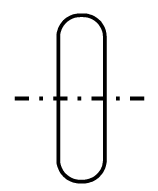
\includegraphics[scale=0.5]{img/simple_non_steering.png}} \\
        \midrule
        {\textsc{Simple steering wheels}}&{Has two axes of rotation, one that is orthogonal to the wheel plane, the other which is \textit{vertical} and goes through the center of the wheel. This provides the wheel with the possibility of changing the orientation with respect to the chassis. Note that for both non-steering and simple steering wheels the component the velocity which orthogonal to the wheel plane is null since there is no sleeping. That is: 
        \begin{equation*}
            v^{\perp}(t)=0
        \end{equation*}}&{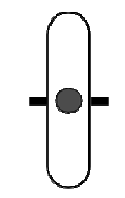
\includegraphics[scale=0.5]{img/simple_steering.png}} \\
        \midrule
        {\textsc{Castor wheel}}&{It is a variant of the previous one in which the vertical axis does not pass through the center of the wheel from which it is \textbf{displaced} by a constant offset. This adds degrees of freedom to the vehicle on which they are mounted on. Such a type of wheels are often used for office chairs and supermarket carts.}&{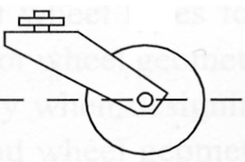
\includegraphics[scale=0.5]{img/castor_wheel.png}} \\
        \midrule
        {\textsc{Omnidirectional or Swedish wheel}}&{There is another type of non-conventional wheel that is the \textit{mechanum} (or \textbf{swedish wheel}). It mounts some passive rollers whose rotation axis is inclined by 45 degrees with respect to the plane of the wheel itself. They are also called \textit{omniwheels}.}&
        {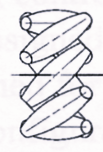
\includegraphics[scale=0.8]{img/swedish_wheel.png}} \\
        \midrule
        {\textsc{Spherical omniwheel}}&{There is another type of omniwheel which is \textbf{spherical}. They can be either active or passive. Like in the case of swedish wheels, a vehicle equipped with four of them is called \textbf{omnidirectional}.}& 
        {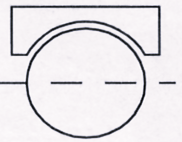
\includegraphics[scale=0.6]{img/spherical_wheel.png}}\\
    \end{tabular}
    \caption{Types of wheels with description and symbols}
    \label{tab:wheels}
\end{table}


\section{Constraints and Kinematic Models}
We have seen in the introduction that mobile and industrial robots have different characteristics, this results in different models, planning and control strategies. Since in general robots are made up of multiple rigid bodies (\textit{multibody system}) linked together by joints, their motion is constrained. This holds in general, however also the types of constraints are different in the case of mobile robots and manipulators. This is because in the former case you have limitations in the \textbf{position} of the whole body, in the case of mobile robots, and in particular in terrestrial wheeled robots, you have instead limitations on \textbf{how the position can change} in magnitude, direction and side (this is nothing but the \textbf{velocity}). From now on we are focusing our attention on \textbf{modeling wheeled robots}.

\subsection{Constraints and their classification}
In order to properly describing and giving a classification of constraints, it is better recalling the concept of \textbf{generalized coordinates}. \\
Let the vector $\mathbf{q}\in\mathbb{R}^n$ be the \emph{generalized coordinates} that describes the \textbf{configuration} of the robot (minimum number of variables needed to model the robot motion). For the moment, let us assume that the \textbf{configuration space} $\mathcal{C}$ coincides with $\mathbb{R}^n$. For example for a \textbf{unicycle} the generalized coordinates are in number of three: 
\begin{equation}\label{eq:gen_coord_unicyle}
    \mathbf{q}=[x \quad y \quad \theta]^T\in\mathbb{R}^3
\end{equation}
where $x$ and $y$ are the position of the contact point between the (single) wheel and the plane on which the motion occurs, while $\theta$ is the angle of the wheel with respect to the horizontal axis. The \textbf{evolution in time} of the generalized coordinates vector \textit{describe the motion} of the system.\\

Constraints can be found by mean of \textbf{equality} (in this case we refer them as \textit{bilateral} constraints), by mean of \textbf{inequality} (we refer them as \textit{unilateral} constraints). Furthermore, according to the fact they are or not time-variant, we can divide them in \textit{rehonomic} (explicit dependence on time) and \textit{scleronomic} (time-invariant constraints). In this course we will treat only \textbf{bilateral and scleronomic constraints} another term for indicating them is \textbf{holonomic} (or \textbf{integrable}) constraints.

\subsubsection{Holonomic constraints}
Such a type of constraint\footnote{
    We recall that for a multibody system described by using the Lagrangian approach, holonomic constraints are those allowing a reduction of the number of needed variables.
} can be expressed as: 

\begin{equation}
    h_i(\mathbf{q})=0, \quad i=1,...,k<n
\end{equation}

A system whose motion is characterized only by holonomic constraints is called \textbf{holonomic system}. By using the \textit{implicit function theorem} (or in Italian "Teorema del Dini"), we can reduce the dimension of the configuration space to $n-k$

\subsubsection{Kinematic constraints}
Such a type of constraints involve both generalized coordinates $\mathbf{q}$ and its derivative $\dot{\mathbf{q}}$. In the most general case they can be expressed as:
\begin{equation}
    a_i(\mathbf{q},\dot{\mathbf{q}})=0, \quad i=1,...,k<n   
\end{equation}
Kinematic constraints are limiting the set of generalized velocities that can be obtained by each configuration. In some cases they can be written in the so-called \textbf{Pfaffian form}, that is they can be written as a \textit{linear combination of the generalized velocities $\dot{\mathbf{q}}$}: 
\begin{equation}
    \mathbf{a}_i^T(\mathbf{q})\dot{{\mathbf{q}}}=0, \quad
    i=1,...,k<n
\end{equation}
An example of kinematic constraint in Pfaffian form is:
\begin{equation*}
    3q_1 \dot{q}_1 +
    2 \sin{q_1}\dot{q_2}+
    \sin{q_3} \dot{q}_3 =0   
\end{equation*}
The reason for using such a notation is that we can immediately retrieve the expression of the associated function by doing the row-by-column product (standard inner product). Such $k$ kinematic constraints can be written in compact form by introducing matrices
\begin{equation}\label{eq:matrix_pfaffian}
    \mathbf{A}^T(\mathbf{q})\dot{\mathbf{q}}=\mathbf{0}
\end{equation}
where $\mathbf{A(q)}\in\mathbb{R}^{k,n}.$ It is interesting to note that the presece of $k$ holonomic constraints imply the presence of $k$ kinematic constraints. This can be easily showed by computing the time derivative for the $k$ holonomic constraints: 
\begin{equation}\label{eq:kin_holonomic}
    \frac{d h_i(\mathbf{q})}{dt}=
    \frac{d h_i(\mathbf{q})}{d\mathbf{q}}\cdot
    \frac{d \mathbf{q}}{dt}=
    \frac{d h_i(\mathbf{q})}{d\mathbf{q}}\cdot \dot{\mathbf{q}}=0, \qquad
    i=1,...,k
\end{equation}
where we have applied the fact that the constraints are holonomic while using the \textit{Chain rule} for passing from the first to the second step. From the \Cref{eq:kin_holonomic} we have understood that: 
\begin{equation*}
    \text{holonomic constraint} \Longrightarrow 
    \text{kinematic constraints}
\end{equation*} 
In general, we cannot say the inverse and in this case (since the step from the derivative to the primitive results in doing the integral) associated constraints are called \textbf{nonholonomic} (or \textbf{non-integrable}) ones. A system characterized by such constraints is called \textbf{nonholonomic system}. In presence of non-integrable constraints the dimension of the configuration space $\mathcal{C}$ cannot be reduced while the generalized velocities can be described over a subspace of dimension $n-k$ (how we are going to see in a minute).

\subsubsection{Example of nonholonomic constraint}
A unicycle rolls on a plane \textbf{without slippering}, we have already seen its generalized coordinates. For such a system we have the so called \textbf{pure rolling constraint}, this imply the velocity of the contact point not to have a non-zero component along the direction orthogonal to the wheels plane. By using simple trigonometric properties involving the inifinitesimal increment $dx$ and $dy$, we can state that
\begin{equation}
    \frac{dy}{dx}=\tan{\theta}
\end{equation}
Can we obtain the Pfaffian form for such a constraint? The answer is YES. In fact by dividing and multiplying for an infinitesimal time increment $dt$ we obtain:
\begin{equation*}
    \frac{dy}{dx}=\frac{dy}{dt}\cdot
    \frac{dt}{dx}=\frac{\dot{y}}{\dot{x}}=\frac{\sin\theta}{\cos{\theta}} \iff 
    \dot{y}\cos{\theta}=\dot{x}\sin{\theta}
\end{equation*}
Which is the same to say that
\begin{equation}
    \dot{x}\sin\theta-\dot{y}\cos{\theta}=0 \iff 
    [\sin\theta \quad \cos\theta \quad 0] \dot{\mathbf{q}}=0
\end{equation}
The constraint we have just derived can be demonstrated that is non-integrable and so nonholonomic, in fact we cannot reduce the dimension of the configuration space (in other words all of the generalized coordinates are needed to properly describe the unicycle motion). Note that, start from an initial state $\mathbf{q}_i$, you can bring the system to any final state $\mathbf{q}_f$, under the assumption of not to violating the pure rolling constraint\footnote{
    We will see that in order to pass from an initial to a final state a \textit{trajectory planning algorithm} must be used.
}.

\subsection{Kinematic model}
From the \Cref{eq:matrix_pfaffian}, we can immediately see that the $n-k$ admissible generalized velocities belong to the null space\footnote{
    Just for doing a brief recap. Given a matrix $A\in\mathbb{R}^{m,n}$ we can individuate the following sets (vector spaces):
    \begin{itemize}
        \itemsep-0.3em
        \item \textsf{Null space} that is the a subset of $\mathbb{R}^n$ defined as: 
        \begin{equation}
            \mathcal{N}(A)=\{x\in\mathbb{R}^n: \ Ax=0\}
        \end{equation}
        \item \textsf{Range space} that is a subset of $\mathbb{R}^m$ defined as: 
        \begin{equation}
            \mathcal{R}(A)=\{y\in\mathbb{R}^m: \ y=Ax\}
        \end{equation}
        the dimension of such a vector space is called the rank of the matrix A (rank(A)) and it holds that its maximum value is the $\min(m,n)$.
    \end{itemize}
    Another important result is that
    \begin{equation*}
        n=\dim{\mathcal{N}(A)}+\dim{\mathcal{R}}(A)
    \end{equation*}
    Knowing $n$ (for us dimension of the configuration space)
 and the rank of A, we can find the dimension for the null space of A.} of $\mathbf{A(q)}^T$ that is 
\begin{equation}
    \dot{\mathbf{q}} \in \mathcal{N}(\mathbf{A^T(q)})
\end{equation}
We know that this is a vector space and it has got a basis of $n-k$ elements which we can denote with $\{\mathbf{g}_i(\mathbf{q})\}_{i=1}^{n-k}$, we can group together such elements in a matrix $\mathbf{G(q)}$ so that the generalized velocities can be expressed as
\begin{equation}
    \mathbf{\dot{q}=G(q)u}
\end{equation}
this is nothing but the \textbf{kinematic model} of the constrained system. The vector $\mathbf{q}$ is called the \emph{state vector} while $\mathbf{u}$ is the \textbf{input vector}. Moreover the obtained system is said to be driftless since in absence of an input the generalized velocity is null. Not rarely the components $u_i$ of \textbf{u} have a meaning related to the physics or the available control input.\\

In the following for better fixing the concepts we have just given, two example of kinematic models are given.

\subsubsection{Kinematic model for the unicycle}
Let us consider, a bit more in details, the unicycle system. It is noticeable that the line in which the motion does not occur is called \textbf{zero motion line}.\\
We have said that the generalized coordinated $\mathbf{q}$ are the ones in \Cref{eq:gen_coord_unicyle}. We have a single constraint that we have reduced in Pfaffian form. The next step \emph{in order to obtain a kinematic model} is determining a base for the null space of the constraint matrix. One possible choice for vector fields $\mathbf{g_i(q)}$ is\footnote{
    Note that this is a vector field since both domain and codomain are vectors of suitable dimensions.
}:
\begin{equation*}
    \mathbf{g}_1(\mathbf{q})=\begin{bmatrix}
        \cos\theta&\sin\theta&0
    \end{bmatrix}^T, \quad
    \mathbf{g}_2(\mathbf{q})=\begin{bmatrix}
        0&0&1
    \end{bmatrix}^T
\end{equation*}
\begin{multicols}{2}
    \noindent
    Therefore, putting them together we obtain the matrix
\begin{equation}
    \mathbf{G(q)}=\begin{bmatrix}
        \cos\theta&0\\
        \sin\theta&0\\
        0&1
    \end{bmatrix}
\end{equation}
The kinematic model for the unicyle, then, can be written as:
\begin{equation}
    \begin{bmatrix}
        \dot{x}\\\dot{y}\\\dot{\theta}
    \end{bmatrix}=\begin{bmatrix}
        \cos\theta\\
        \sin\theta\\
        0
    \end{bmatrix}v+\begin{bmatrix}
        0\\0\\1
    \end{bmatrix}\omega
\end{equation}
\\
\begin{figure}[H]
    \centering
    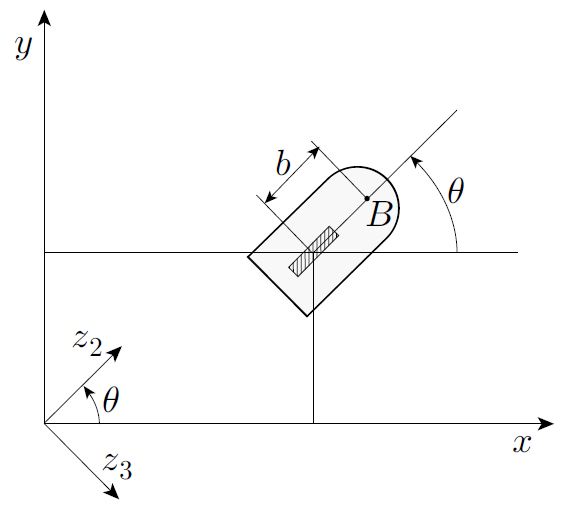
\includegraphics[scale=0.6]{img/unicycle_scheme.png}
    \caption{Choice of generalized coordinates for the unicycle}
    \label{fig:unicycle_model}
\end{figure}
\end{multicols}
In such a context the elements of the input vector have a physical meaning, since $v$ is the driving velocity, while $\omega$ is nothing but the steering velocity.  Why are we interested in studying the kinematic model of a unicyle? Consider that without a human beings balancing the system this is also an unstable system! However, there are some robot (stable) robot structures that from a \textbf{kinematic point of view} are equivalent to unicycles. We are talking about \emph{differential drive} and \emph{synchro drive} vehicles.

\subsubsection{Kinematic model for a bicycle}
A \textbf{bicycle} is vehicle with a steered wheel and a fixed one, the distance between the wheels is fixed to be $L$. As usual we have to choose the (generalized) coordinates for such a vehicle a possible choice is the following:
\begin{itemize}
    \itemsep-0.3em
    \item $(x,y)$ being the contact point of the rear\footnote{
        back wheel
    }; 
    \item $\theta$ is the angle between the rear wheel and the $x$ axis (this is nothing but the orientation of the vehicle with respect to the $x$ axis); 
    \item $\phi$ is the steering angle of the front wheel.
\end{itemize}
\begin{remark}
    It is interesting focus our attention on a point: why do not we introduce also the coordinates of the front wheel? Well, it is sufficient having a single contact point since, back and front wheel are at a fixed distance $\ell$, and this is nothing but an \textit{holonomic constraint} which allows us the shrinking of the configuration space dimension! 
\end{remark}
Going on into the discussion, there are essentially two \textit{pure rolling constraints}, one for each wheel: 
\begin{align}
    &\dot{x}_f \sin(\theta+\phi)-\dot{y}_f \cos(\theta+\phi)=0 \label{eq:front_pure_rolling}\\
    &\dot{x}\sin(\theta)-\dot{y}\cos(\theta)=0
\end{align}
while indicating with $(x_f,y_f)$ the coordinates of the front wheel center, while $(\theta+\phi)$ is its angle with respect to the fixed reference frame. We have just said that they are not strictly necessary, since they can be obtained starting from the coordinates of the other wheel in particular: 
\begin{equation}
    \begin{cases}
        x_f=x+\ell\cos\theta\\
        y_f=y+\ell\sin\theta
    \end{cases}
\end{equation} 
using the trigonometry, the \Cref{eq:front_pure_rolling} can be expressed as
\begin{equation}
    \dot{x}\sin(\theta+\phi)-\dot{y}\cos(\theta+\phi)-\ell\dot{\theta}\cos(\phi)=0
\end{equation}
where we have used that $\sin^2\theta+\cos^2\theta=1$ and the trigonometric formulas for $\cos(\theta+\phi)$ and $\sin(\theta+\phi)$. The derived constraints can be put if Pfaffian form using the matrix
\begin{equation}
    \mathbf{A}^T(\mathbf{q})=\begin{bmatrix}
        \sin\theta&-\cos\theta&0&0\\
        \sin(\theta+\phi)&-cos(\theta+\phi)&-\ell\cos\phi&0
    \end{bmatrix}
\end{equation}
\begin{multicols}{2}
    
\noindent 
Our objective is obtaining a basis for the null space of such a matrix in order to derive the kinematic model. Since $rank(\mathbf{A^T(q)})=2$, the dimension of its null space is given by the difference between the dimension of the configuration space and such a rank, that is 2. A possible basis for such a null space is given by the column of
\begin{equation}
    \mathbf{G(q)}=\begin{bmatrix}
        \cos\theta\cos\phi&0\\
        \sin\theta\cos\phi&0\\
        \frac{\sin\theta}{\ell}&0\\
        0&1
    \end{bmatrix}
\end{equation}
\begin{figure}[H]
    \centering
    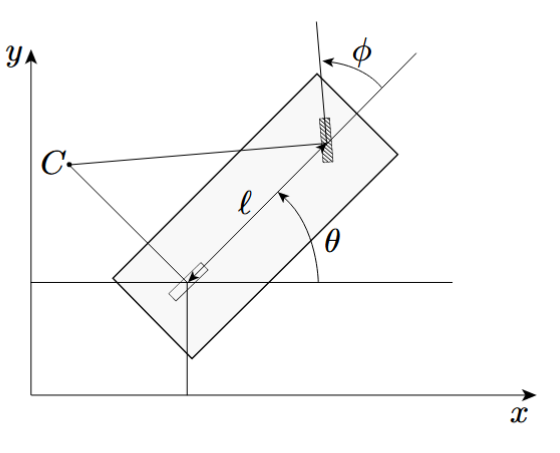
\includegraphics[scale=0.6]{img/bicycle_scheme.png}
    \caption{Possible choice for the generalized coordinates of a unicycle}    
    \label{fig:scheme_bicycle}
\end{figure}
\end{multicols}
\noindent
The associated kinematic model is:
\begin{equation}
    \begin{bmatrix}
        \dot{x}\\
        \dot{y}\\
        \dot{\theta}\\
        \dot{\phi}
    \end{bmatrix}=\begin{bmatrix}
        \cos\theta\cos\phi\\
        \sin\theta\cos\phi\\
        \frac{\sin\theta}{\ell}\\
        0
    \end{bmatrix}u_1 + \begin{bmatrix}
        0\\
        0\\
        0\\1
    \end{bmatrix}\omega
\end{equation}
the control input $u_1$ can be choosen according to the drive in particular $u_1=v$ if the vehicle is front-drive, $u_1=v/\cos\theta$ if the vehicle is back drive, since the first two equations must be equivalent to the ones of a unicyle. Just for a matter of notation/nomenclature the instersection point $C$ between the two zero motion lines is called \textit{instantaneous center of rotation}, depends only on $\mathbf{q}$ and it is interesting since each point of the chassis is moving instantaneously along along the circumference centered at $C$ (see \Cref{fig:scheme_bicycle}).\\
Equivalent (stable) systems having the same kinematic model are the \textbf{tricyle} and the \textbf{automobile}.

\section{Sensors for mobile robots}

